\documentclass{article}
\usepackage{amsmath}
\usepackage{graphicx}
\begin{document}
\title{Equations of Lines: Question 11}
\author{Ana Bhattacharjee}
\date{\today}
\maketitle
\begin{center}
Below is a picture of the right triangle.
\begin{figure}[!htbp]
  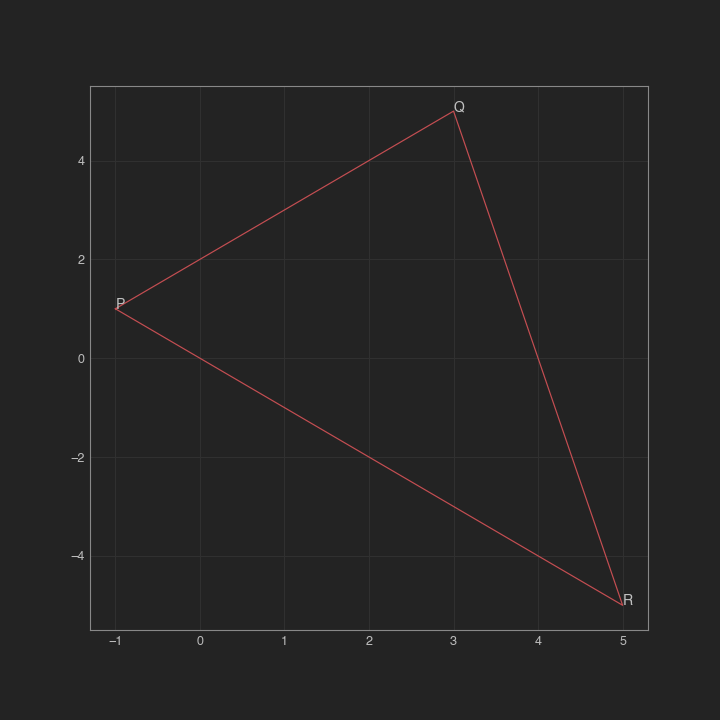
\includegraphics[width=1.1\columnwidth]{../line_eq_q11}
  \caption{Right Triangle}
\end{figure}
The first step is to find the slope of base QR. Then the slope of the altitude will be perpendicular to QR. The equation of the line will contain point P.
\begin{align}
Q (3,5) \\
R (5, -5) \\
\text{slope} = \frac{-5 - 5}{5 - 3} = -5 \\
\text{perpendicular\_slope} = -5x = -1 \rightarrow \frac{-x}{5} = \frac{-1}{-5} \rightarrow x = \frac{1}{5} \\
y = mx + b \\
P (-1, 1) \\
y = \frac{1}{5}x + b \\
1 = \frac{-1}{5} + b \\
1 + \frac{1}{5} = b \\
b = \frac{6}{5}
\end{align}
\end{center}
\end{document}
